\section{Prompt Engineering\\{\small Tecniche di base}}
\label{sec:pe_base}
%
\begin{frame}[t] \frametitle{\emph{Prompt Engineering}}
\framesubtitle{Definizione}
{\small
\onslide<1->
    \begin{minipage}[t]{\textwidth}
        \vspace*{-.5cm}
        \begin{figure}
            \centering
            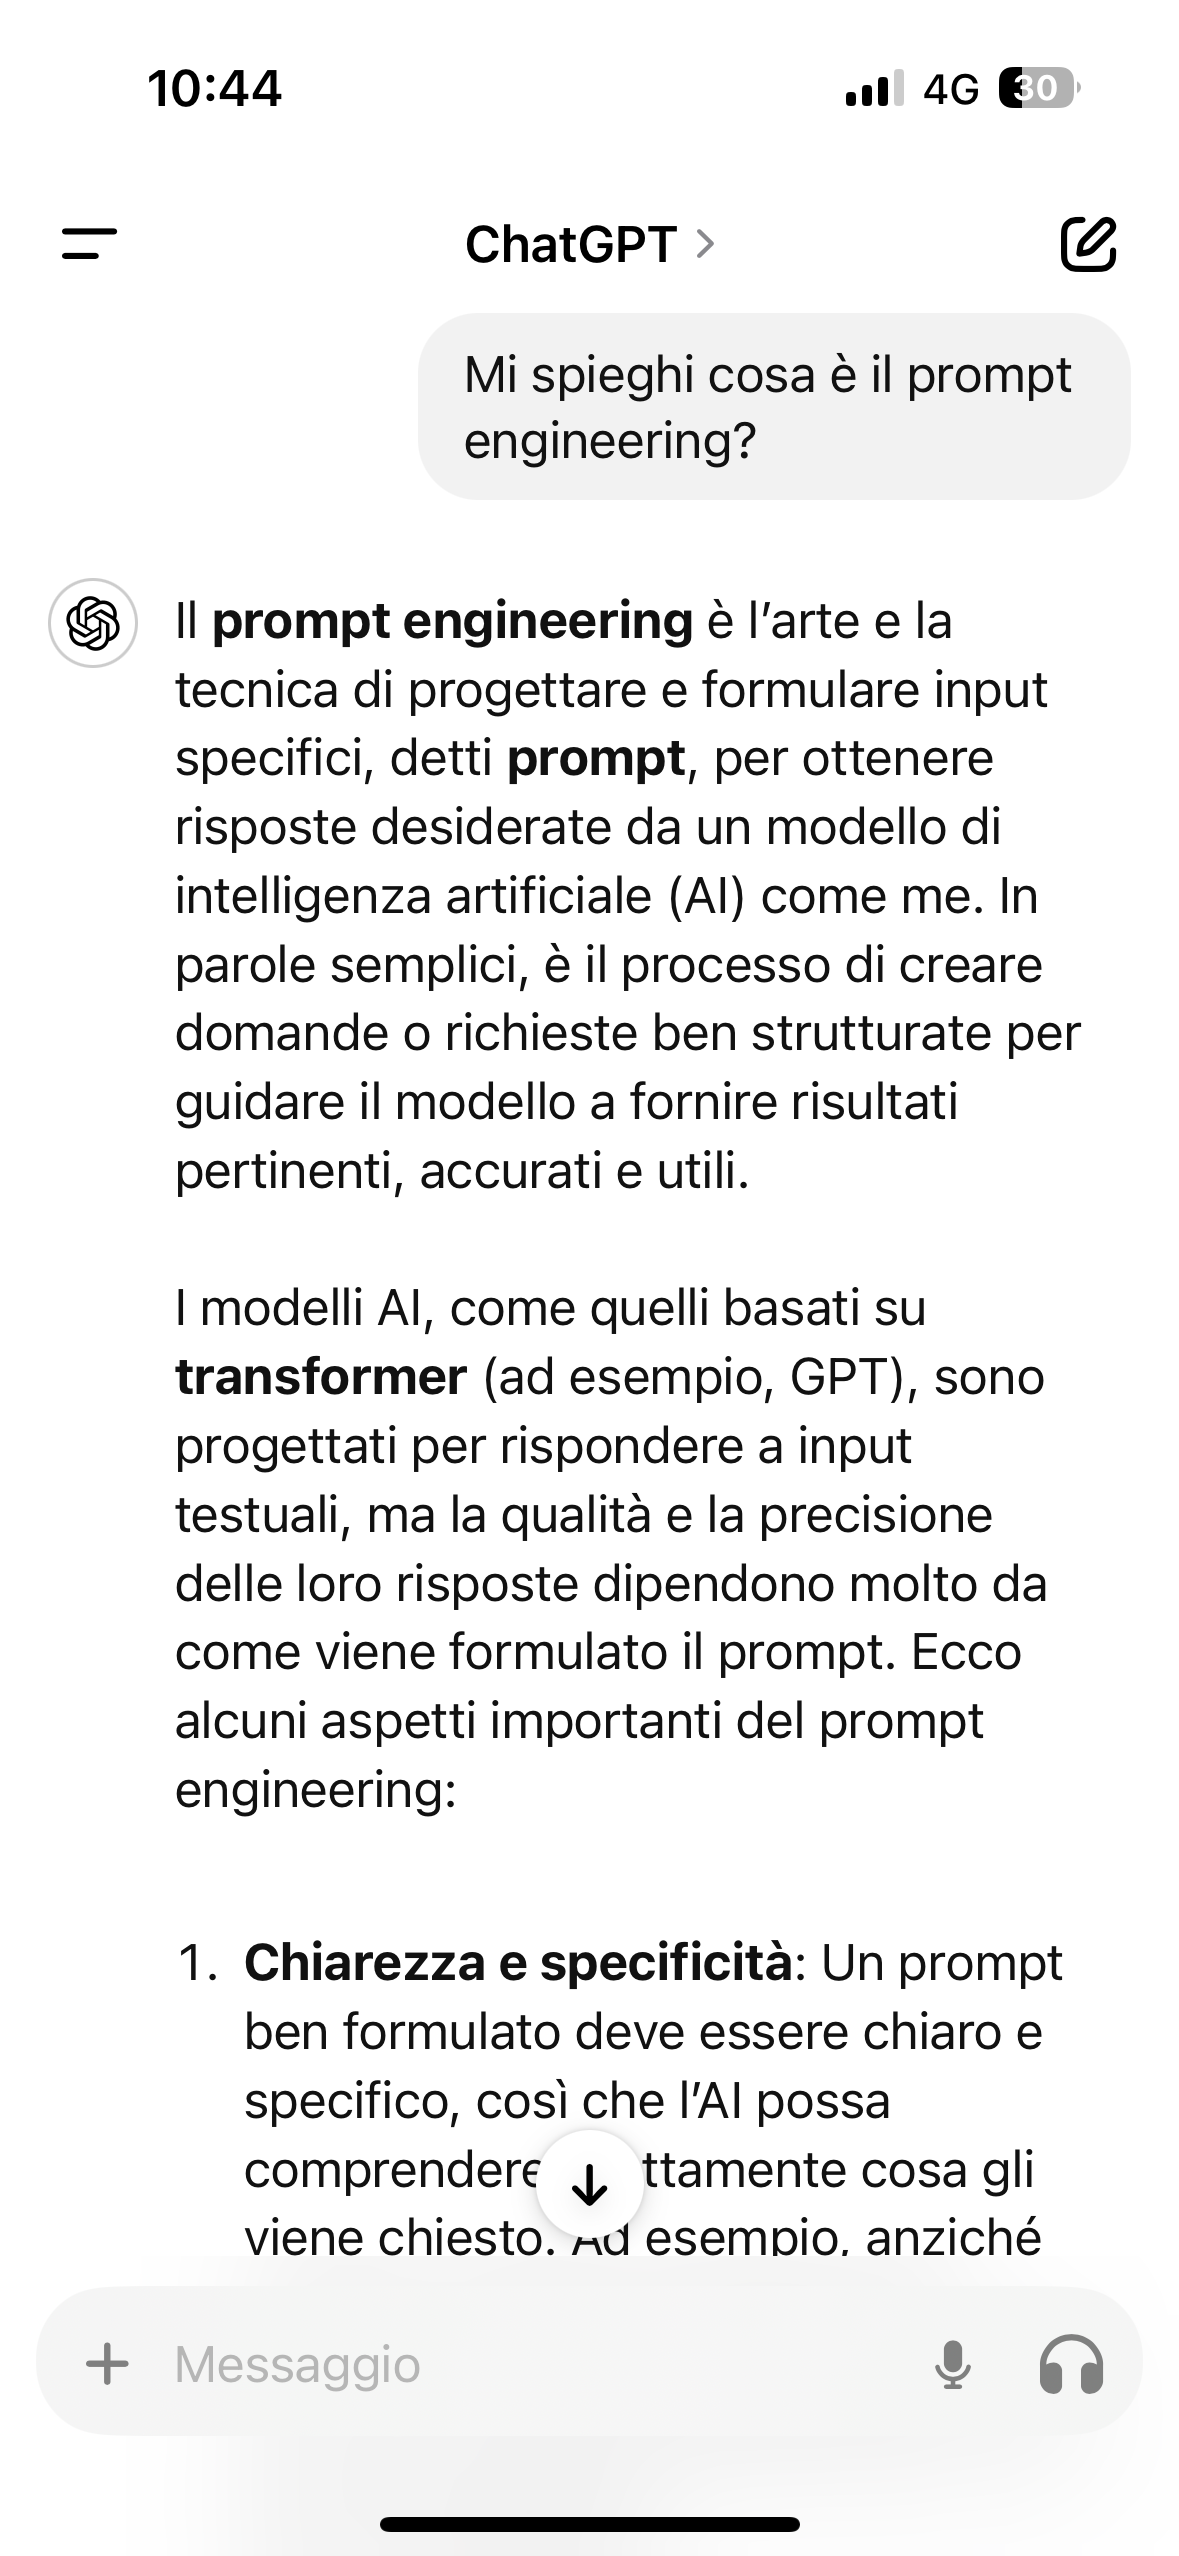
\includegraphics[width=.25\textwidth]{img/PE-1.PNG}
            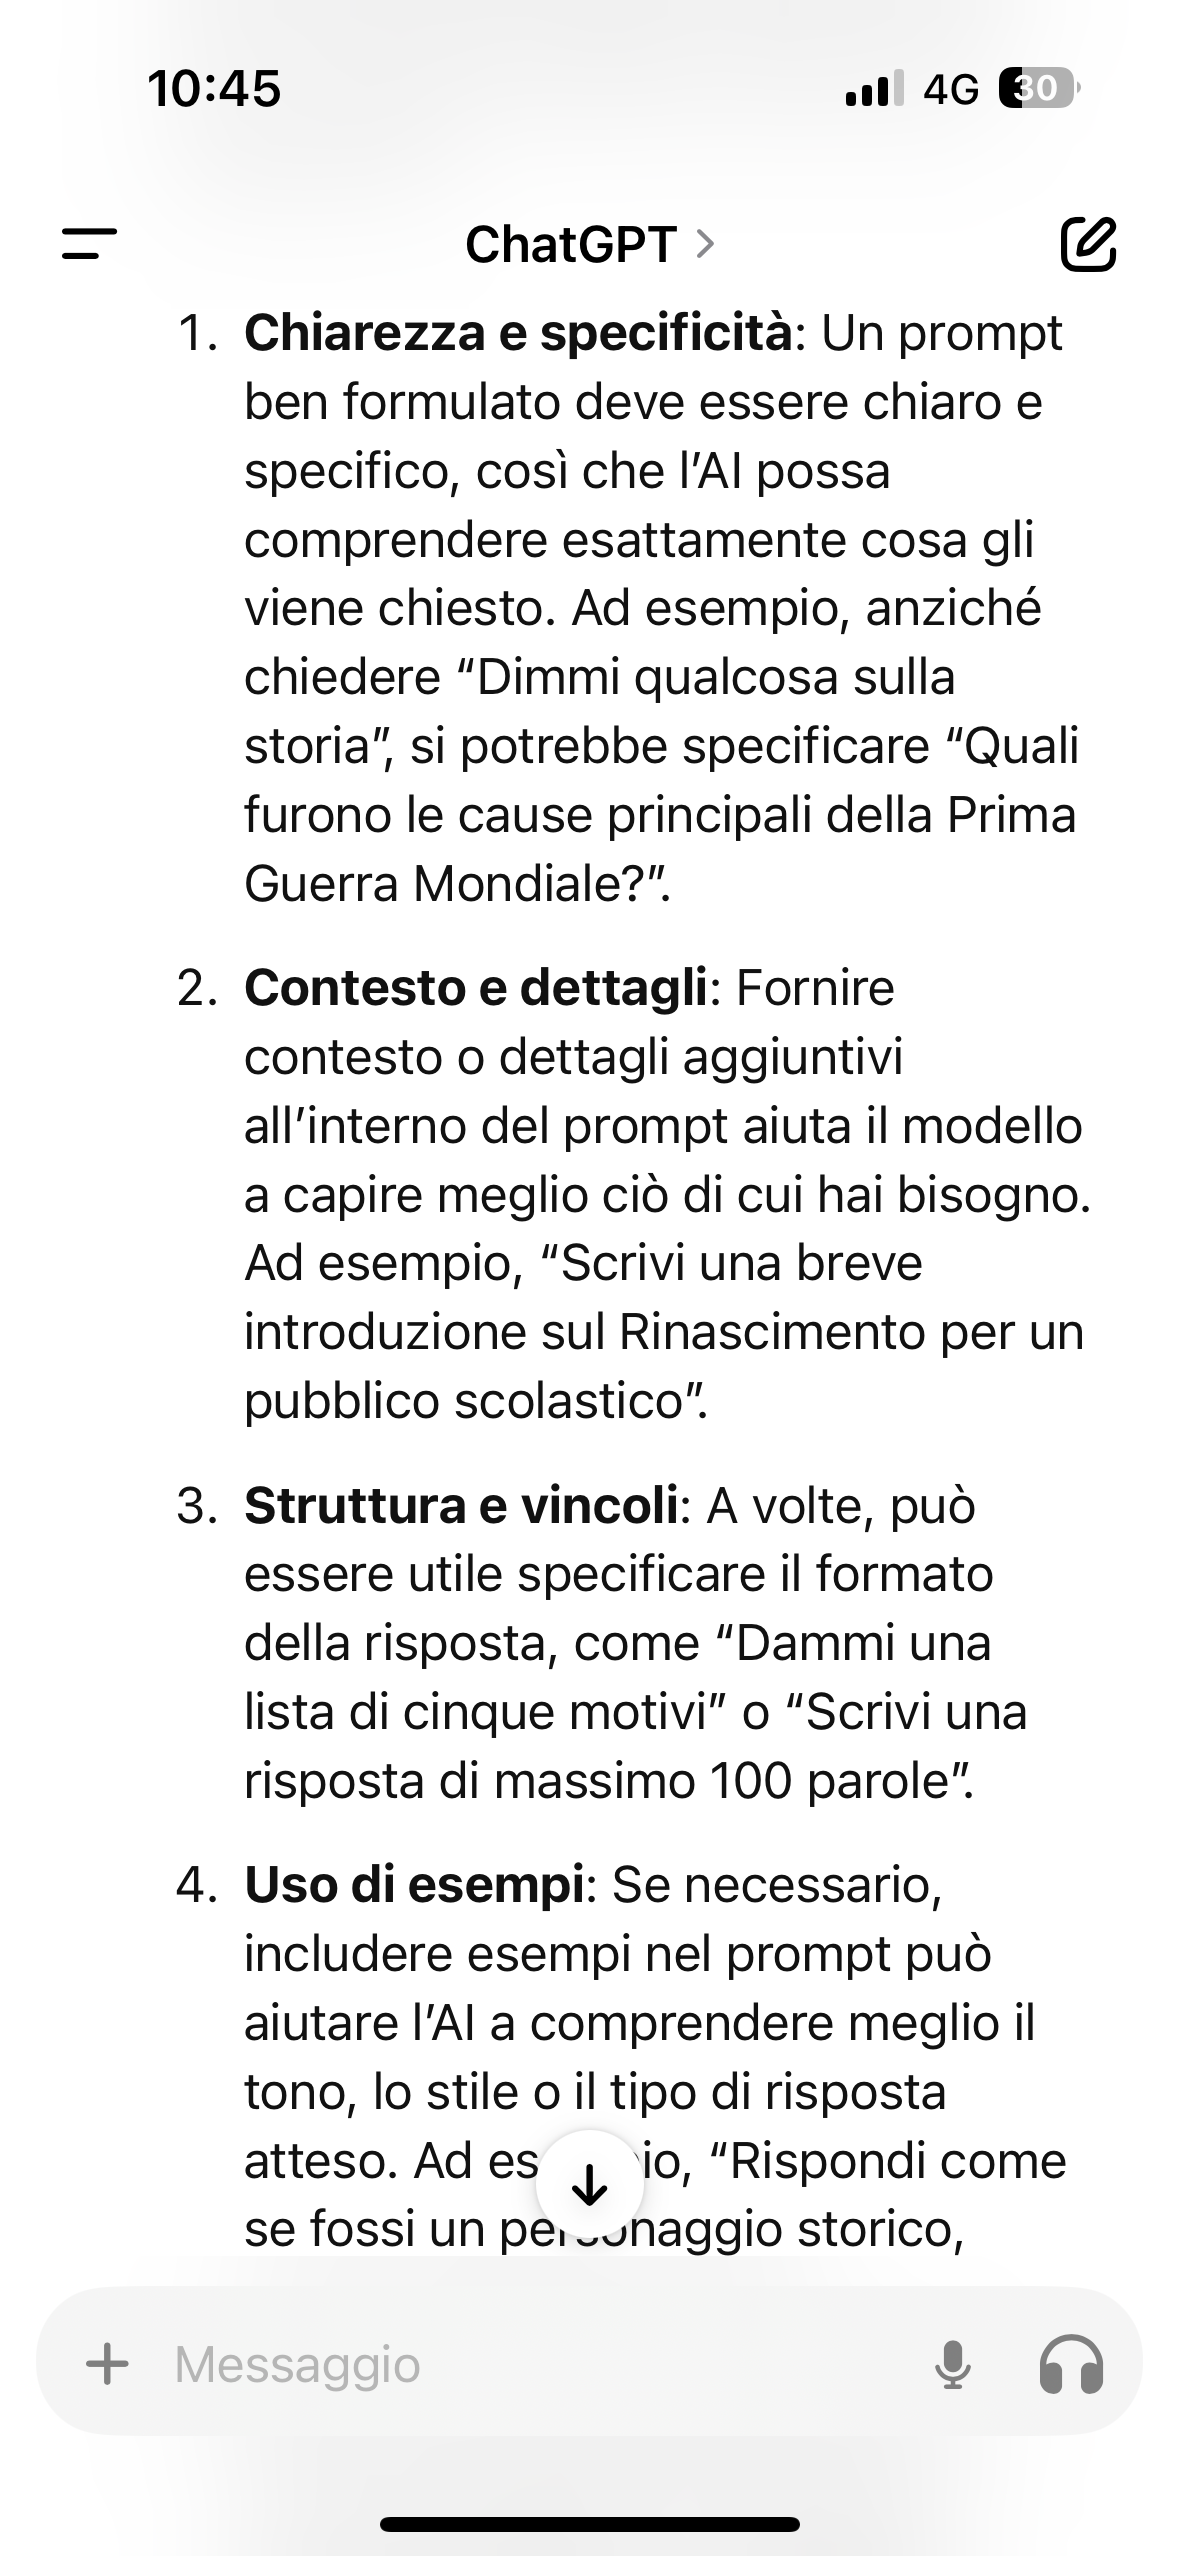
\includegraphics[width=.25\textwidth]{img/PE-2.PNG}
            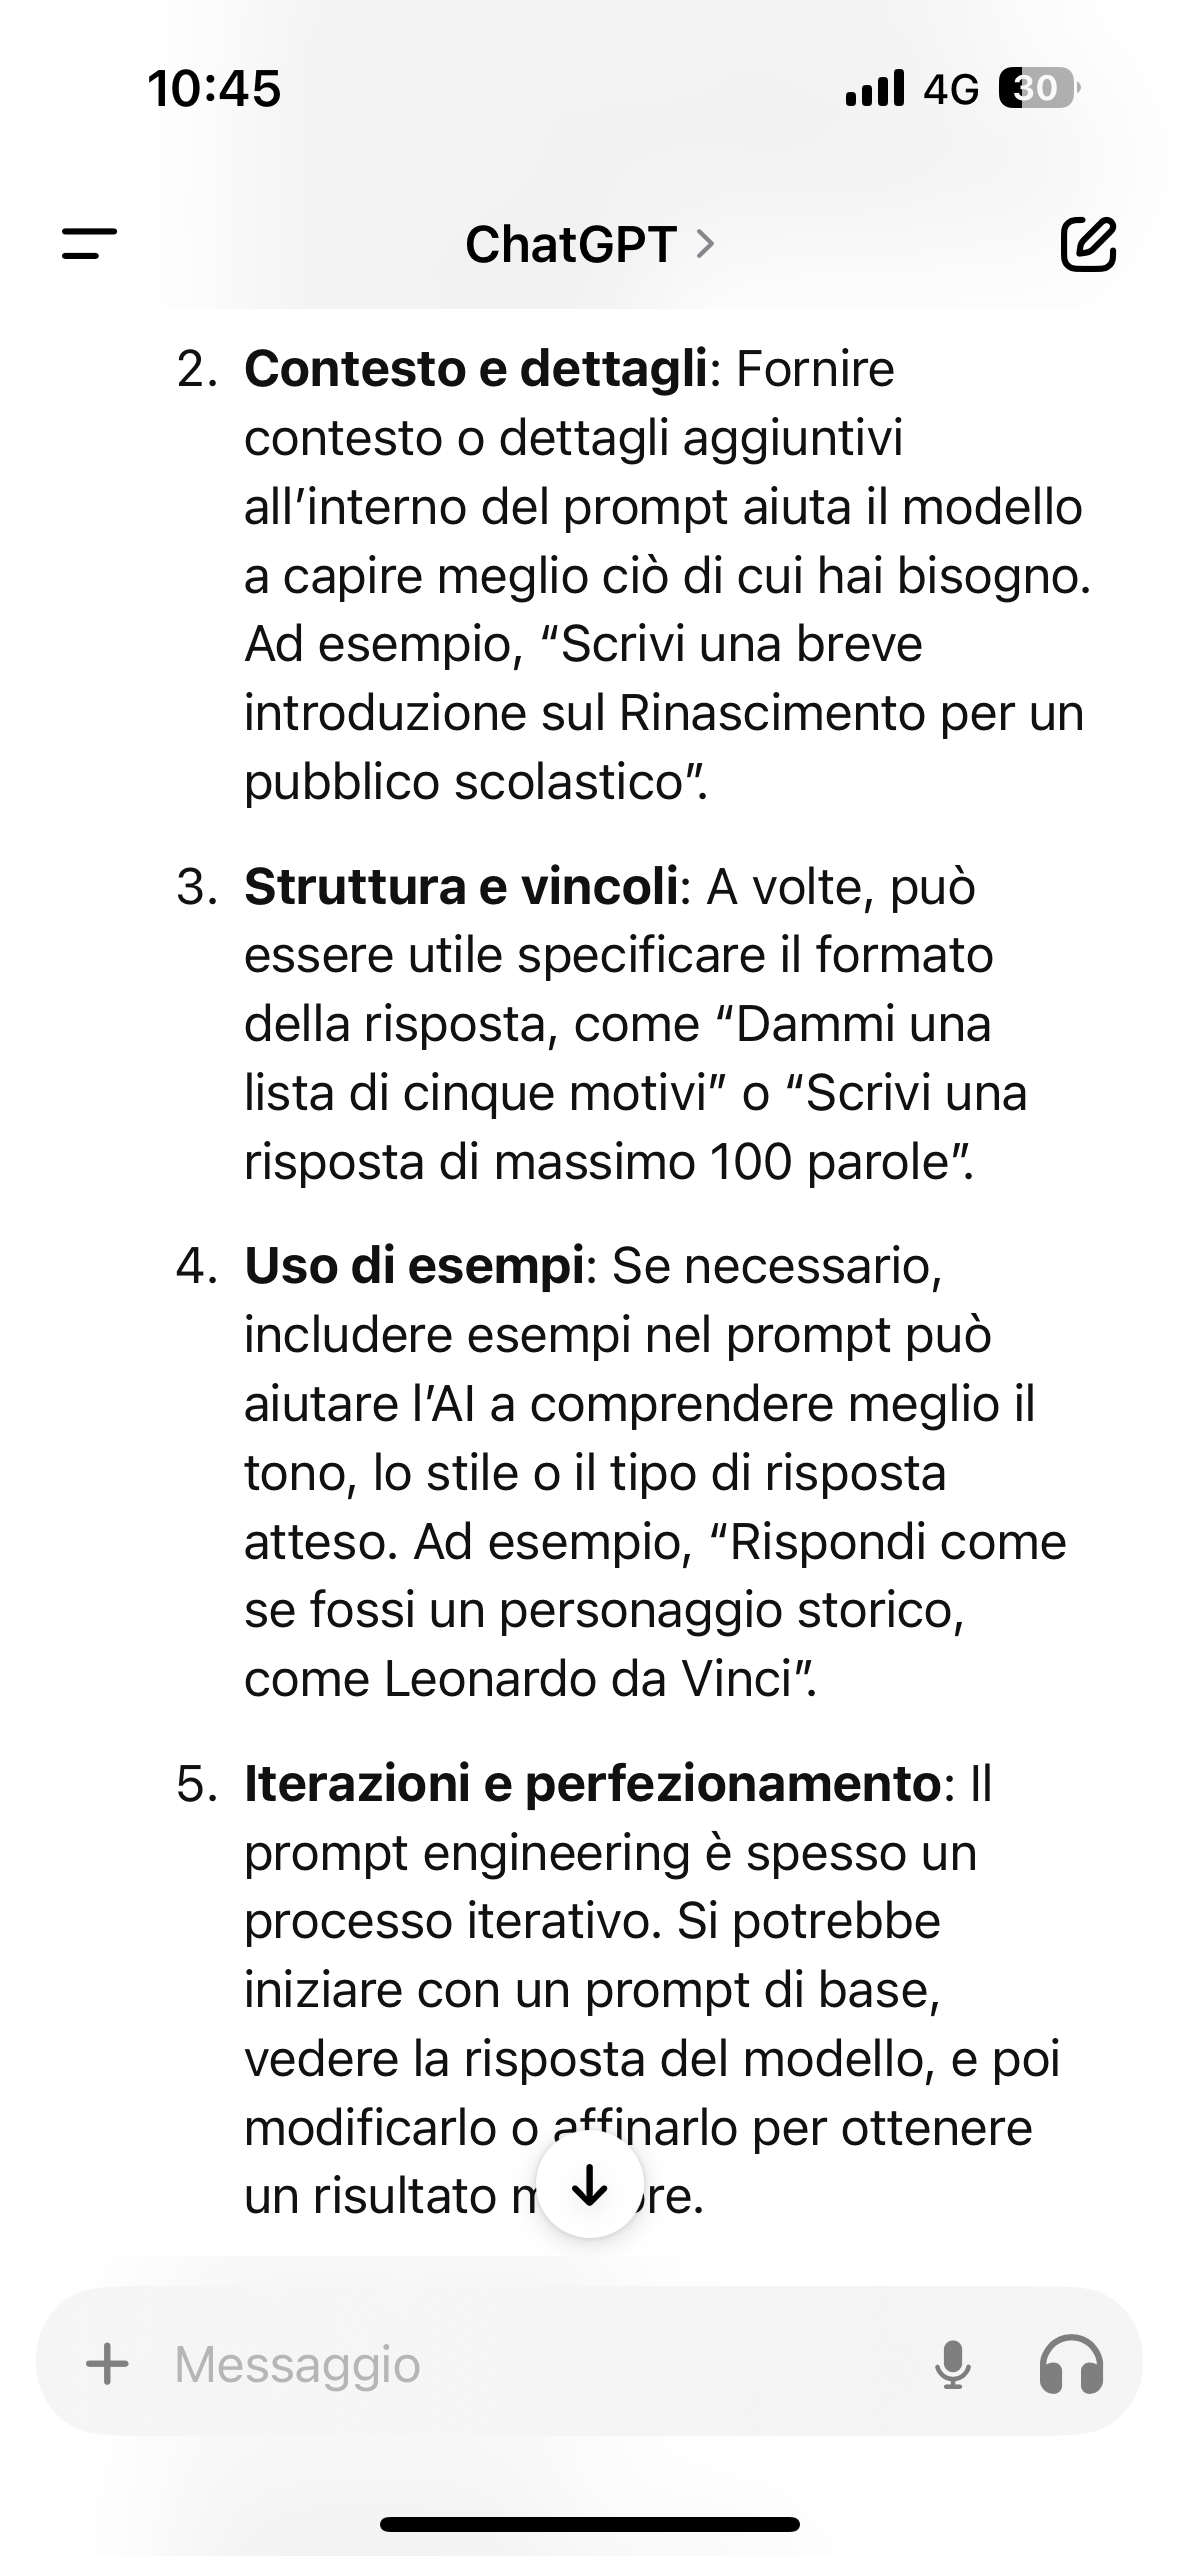
\includegraphics[width=.25\textwidth]{img/PE-3.PNG}
        \end{figure}
    \end{minipage}
    \\\vspace*{.3cm}
    \begin{minipage}[t]{\textwidth}
        \begin{itemize}[leftmargin=10pt,align=right]
            \onslide<1->\item[\alert{\faArrowCircleRight}] Definiamo meglio il concetto di \emph{prompt}$\ldots$
        \end{itemize}
    \end{minipage}
}
\end{frame}
%
\begin{frame}[t] \frametitle{\emph{Prompt Engineering}}
\framesubtitle{Il perfetto prompt engineer}
	{\footnotesize
	    \begin{minipage}[t]{\textwidth}
			\begin{minipage}[t]{0.6\textwidth}
	    		\begin{itemize}[leftmargin=10pt,align=right]
					\onslide<1->\item[\alert{\faArrowCircleRight}] Sceglie uno \alert{specifico} modello da ottimizzare
					\onslide<2->\item[\alert{\faArrowCircleRight}] Capisce come è stato addestrato il modello
					\onslide<3->\item[\alert{\faArrowCircleRight}] Capisce come è stato configurato il modello
                    \onslide<4->\item[\alert{\faArrowCircleRight}] Comprende come riconfigurare il modello
					\onslide<5->\item[\alert{\faArrowCircleRight}] Si esprime efficacemente con il modello
                    \begin{itemize}[leftmargin=10pt,align=right]
                        \item[\alert{\faArrowCircleRight}] Stile
                        \item[\alert{\faArrowCircleRight}] Tono
                        \item[\alert{\faArrowCircleRight}] Struttura
                        \item[\alert{\faArrowCircleRight}] Scelta delle parole
                    \end{itemize}
                    \onslide<6->\item[\alert{\faExclamationTriangle}] Spinge il LLM verso un comportamento \alert{pseudo-deterministico}  
				\end{itemize}
            \end{minipage}
            %
			\hfill
            \onslide<1->
            \begin{minipage}[t]{0.4\textwidth}
                \centering
                \begin{figure}[ht]
                    
\includegraphics[width=\textwidth]{the-mentalist.jpg}
                    {\tiny\\The Mentalist\\\vspace*{-1pt}\textit{\textcopyright Prime Video}}
                \end{figure}
            \end{minipage}
	    \end{minipage}
	}
\end{frame}
%
\begin{frame}[t] \frametitle{\emph{Prompt Engineering}}
\framesubtitle{Controlli di output LLM - I}
{\small
    \begin{minipage}[t]{\textwidth}
        \begin{itemize}[leftmargin=10pt,align=right]
            \onslide<1->\item[\alertedcircled{1}] \alert{Lunghezza massima:} numero di \emph{token} massimo generato dal modello
            \begin{itemize}[leftmargin=10pt,align=right]
                \onslide<2->\item[\alert{\faArrowCircleRight}] Evitare alti consumi (energetici, economici, \ldots)
                \onslide<3->\item[\alert{\faArrowCircleRight}] Abbattere i tempi di risposta
                \onslide<4->\item[\alert{\faArrowCircleRight}] Cruciale in alcuni tipi di strategie di \textit{prompting} (ReAct) e per alcune tipologie di \textit{task}
                \onslide<5->\item[\alert{\faExclamationTriangle}] \alert{Non} impone modifiche stilistiche al modello!
            \end{itemize}
        \end{itemize}
    \end{minipage}
}
\end{frame}
%
\begin{frame}[t] \frametitle{\emph{Prompt Engineering}}
\framesubtitle{Controlli di output LLM - II}
{\footnotesize
    \begin{minipage}[t]{\textwidth}
        \begin{itemize}[leftmargin=10pt,align=right]
            \onslide<1->\item[\alertedcircled{2}] \alert{Creatività del modello:} libertà nella scelta del \emph{token} successivo
            \begin{itemize}[leftmargin=10pt,align=right]
                \onslide<2->\item[\alert{\faArrowCircleRight}] \alert{Temperatura:}
                \begin{itemize}[leftmargin=10pt,align=right]
                    \item[\alert{\faArrowCircleRight}] \alert{Bassa} se vogliamo risposte più deterministiche
                    \item[\alert{\faArrowCircleRight}] \alert{Alta} per risposte ``creative''
                    \item[\alert{\faExclamationTriangle}] Intervallo $[0, +\infty]$
                \end{itemize}
                \onslide<3->\item[\alert{\faArrowCircleRight}] \alert{Top-K:} seleziona i primi K \textit{token} più probabili dalla distribuzione
                 \begin{itemize}[leftmargin=10pt,align=right]
                    \item[\alert{\faExclamationTriangle}] Intervallo $[0, +\infty]$
                \end{itemize}               
                \onslide<4->\item[\alert{\faArrowCircleRight}] \alert{Top-P:} seleziona i \textit{token} più probabili e la cui probabilità cumulativa non supera P
                  \begin{itemize}[leftmargin=10pt,align=right]
                    \item[\alert{\faExclamationTriangle}] Intervallo $[0, 1]$
                \end{itemize}                    
                \onslide<5->\item[\alert{\faExclamationTriangle}] Non sempre tutti disponibili!
                \begin{itemize}[leftmargin=10pt,align=right]
                    \item[\alert{\faArrowCircleRight}] Se tutte disponibili, Top-K e Top-P scremano, temperatura decide
                    \item[\alert{\faArrowCircleRight}] Se temperatura manca, Top-K e Top-P scremano, processo \textit{random} decide
                \end{itemize}
            \end{itemize}
        \end{itemize}
    \end{minipage}
}
\end{frame}
%
\begin{frame}[t] \frametitle{\emph{Prompt Engineering}}
\framesubtitle{Come bilanciare temperatura, Top-P, Top-K?}
	{\small
	    \begin{minipage}[t]{\textwidth}
			\begin{minipage}[t]{0.55\textwidth}
	    		\begin{itemize}[leftmargin=10pt,align=right]
					\onslide<1->\item[\alert{\faArrowCircleRight}] Attenzione alle configurazioni \textit{borderline}
                \end{itemize}    
                {\tiny
                    \begin{table}
                    %% increase table row spacing, adjust to taste
                    \renewcommand{\arraystretch}{1}
                    \centering
                    \begin{tabularx}{\textwidth}{p{.2\textwidth}p{.7\textwidth}}
                        \toprule
                        \textbf{\emph{Setup}} & \textbf{Effetto}\\
                        \midrule
                        Temp $=$ 0 & Top-P, Top-K irrilevanti (\alert{\textit{greedy decoding}})\\
                        Temp $\gg$ 0 & Temp irrilevante\\
                        \midrule
                        Top-K $=$ 1 & Temp, Top-P irrilevanti (\alert{\textit{greedy decoding}})\\
                        Top-K $\gg$ 1 & Decide Temp ma processo decisamente \textit{random}\\
                        \midrule
                        Top-P $=$ 0 & Temp, Top-K irrilevanti (per maggioranza dei modelli)\\
                        Top-P $=$ 1 & Top-P irrilevante\\
                        \bottomrule
                    \end{tabularx}
                    \end{table}
                }
            \end{minipage}
            %
			\hfill
            \onslide<1->
            \begin{minipage}[t]{0.38\textwidth}
                \centering
                \begin{figure}[ht]
                    
\includegraphics[width=\textwidth]{yzma-cronk.jpg}
                    {\tiny\\Yzma e Kronk\\\vspace*{-1pt}\textit{\textcopyright Disney}}
                \end{figure}
            \end{minipage}
	    \end{minipage}
        \begin{itemize}[leftmargin=10pt,align=right]
			\onslide<2->\item[\alert{\faArrowCircleRight}] Per iniziare (secondo Google)               
        \end{itemize}
        \begin{minipage}[t]{0.65\textwidth}
        {\footnotesize
            \begin{table}
            %% increase table row spacing, adjust to taste
            \renewcommand{\arraystretch}{1}
            \centering
            \begin{tabularx}{\textwidth}{llll}
                \toprule
                \textbf{Obiettivo} & \textbf{Temp} & \textbf{Top-P} & \textbf{Top-K}\\
                \midrule
                Risposte formali        & .2 & .95 & 30  \\
                Risposte creative       & .1 & .9  & 20  \\
                Risposte molto creative & .9 & .99 & 40  \\
                Risposta matematica     & 0  & --- & --- \\
                \bottomrule
            \end{tabularx}
            \end{table}
        }
        \end{minipage}
	}
\end{frame}
%
\begin{frame}[t] \frametitle{\emph{Prompt Engineering}}
\framesubtitle{Controlli di output LLM - III}
{\small
    \begin{minipage}[t]{\textwidth}
        \begin{itemize}[leftmargin=10pt,align=right]
            \onslide<1->\item[\alertedcircled{3}] \alert{Sequenze di terminazione:} bloccano la terminazione della generazione
            \begin{itemize}[leftmargin=10pt,align=right]
                \onslide<2->\item[\alert{\faArrowCircleRight}] Generazione di una lista di non più di 10 punti $\leadsto$ \texttt{stop\_sequence=[11]}     
            \end{itemize}
            \onslide<3->\item[\alertedcircled{4}] \alert{Penalità di ripetizione:} incentivare il modello a sfruttare la ricchezza del suo dizionario
            \begin{itemize}[leftmargin=10pt,align=right]
                \onslide<4->\item[\alert{\faArrowCircleRight}] \alert{\textit{Frequency penalty:}} penalità calcolata su ciascun \textit{token} proporzionale al numero di apparizioni nella sequenza generata
                \onslide<5->\item[\alert{\faArrowCircleRight}] \alert{\textit{Presence penalty:}} penalità \alert{globale} indipendente da \textit{token} o numero di occorrenze
            \end{itemize}
        \end{itemize}
    \end{minipage}
}
\end{frame}
%
\begin{frame}[t] \frametitle{\emph{Prompt Engineering}}
\framesubtitle{Componenti principali}
{\small
\onslide<1->
    \begin{minipage}[t]{\textwidth}
        \begin{itemize}[leftmargin=70pt,align=right]
            \onslide<1->\item[\alert{Direttive}] istruzioni specifiche relative alla \textit{task} da eseguire
            \onslide<2->\item[\alert{Esempi}] per guidare il LLM verso un \textit{output} più efficace
            \onslide<3->\item[\alert{Ruolo (persona)}] la prospettiva che il LLM deve adottare per definire tono, stile e contenuto della risposta
            \onslide<4->\item[\alert{``Contesto''}] informazioni aggiuntive che possono indirizzare e addestrare il modello in modo che generi risposte migliori, pertinenti e coerenti con l'obiettivo
            \onslide<5->\item[\alert{Dati di \emph{input}}] il testo contenente l'istanza della \textit{task} da risolvere
            \onslide<6->\item[\alert{Indicatore di \emph{output}}] la tipologia o il formato che si vuole ottenere nella risposta
        \end{itemize}
        \vspace*{.5cm}
        \begin{itemize}[leftmargin=10pt,align=right]
            \onslide<7->\item[\alert{\faArrowCircleRight}] Dati di \emph{input} obbligatori
            \onslide<8->\item[\alert{\faArrowCircleRight}] Altri dati opzionali
        \end{itemize}
    \end{minipage}
}
\end{frame}
%
\begin{frame}[t] \frametitle{\emph{Prompt Engineering}}
\framesubtitle{Best practice per componente - I}
\vspace*{-15pt}
{\small
\onslide<1->
    \begin{minipage}[t]{\textwidth}
        \begin{itemize}[leftmargin=10pt,align=right]
            \onslide<1->\item[\alert{\faArrowCircleRight}] Direttive
            \begin{itemize}[leftmargin=10pt,align=right]
                \item[\alert{\faExclamationTriangle}] Essere chiari e concisi
                \item[\alert{\faExclamationTriangle}] Evitare istruzioni ambigue e vaghe
                \item[\alert{\faExclamationTriangle}] Quando possibile, utilizzare verbi che decrivono le azioni da eseguire (``Traduci'', ``Fai una lista di \ldots'')
            \end{itemize}
            \onslide<2->\item[\alert{\faArrowCircleRight}] Esempi
            \begin{itemize}[leftmargin=10pt,align=right]
                \item[\alert{\faExclamationTriangle}] Chiari e rilevanti per la \textit{task}
                \item[\alert{\faExclamationTriangle}] Mostrare la struttura o contenuto atteso
                \item[\alert{\faExclamationTriangle}] Numero di esempi comminato alla complessità della \textit{task}
            \end{itemize}
            \onslide<3->\item[\alert{\faArrowCircleRight}] Ruolo (persona)
            \begin{itemize}[leftmargin=10pt,align=right]
                \item[\alert{\faExclamationTriangle}] Aggiungere \textit{expertise} o una prospettiva specifica
                \item[\alert{\faExclamationTriangle}] Ruolo allineato alla \textit{task} (es., esperto di \textit{marketing} per generare contenuto promozionale)
                \item[\alert{\faExclamationTriangle}] Combinare ruolo con il ``contesto''
            \end{itemize}
        \end{itemize}        
    \end{minipage}
}
\end{frame}
%
\begin{frame}[t] \frametitle{\emph{Prompt Engineering}}
\framesubtitle{Best practice per componente - II}
\vspace*{-15pt}
{\small
\onslide<1->
    \begin{minipage}[t]{\textwidth}
        \begin{itemize}[leftmargin=10pt,align=right]
            \onslide<1->\item[\alert{\faArrowCircleRight}] Contesto
            \begin{itemize}[leftmargin=10pt,align=right]
                \item[\alert{\faExclamationTriangle}] Includere informazione strettamente rilevante
                \item[\alert{\faExclamationTriangle}] Informazione strettamente collegata alla \textit{task}
                \item[\alert{\faExclamationTriangle}] Fornire un \textit{background}, soprattutto in sotto-casi specifici
            \end{itemize}
            \onslide<2->\item[\alert{\faArrowCircleRight}] Indicatore di \textit{output}
            \begin{itemize}[leftmargin=10pt,align=right]
                \item[\alert{\faExclamationTriangle}] Se possibile, sfruttare meccanismi automatici ottimizzati (es. \texttt{BeanOutputConverter} in Spring AI)
            \end{itemize}
        \end{itemize}        
    \end{minipage}
}
\end{frame}
%
\begin{frame}[t] \frametitle{\emph{Prompt Engineering}}
\framesubtitle{Esiste un ordine?}
{\normalsize
    \begin{minipage}[t]{\textwidth}
        \begin{itemize}[leftmargin=10pt,align=right]
            \onslide<1->\item[\alertedcircled{1}] Esempi (se necessari)
            \onslide<2->\item[\alertedcircled{2}] ``Contesto'' (informazioni aggiuntive)
            \onslide<3->\item[\alertedcircled{3}] Ruolo (persona)
            \onslide<4->\item[\alertedcircled{4}] Direttive
            \onslide<5->\item[\alertedcircled{5}] Dati di \textit{input}
            \onslide<6->\item[\alertedcircled{6}] Indicatore di \textit{output}
        \end{itemize}        
    \end{minipage}
    \onslide<7->
    \begin{itemize}[leftmargin=10pt,align=right]
        \item[\alert{\faExclamationTriangle}] Evitare che LLM generi \alert{ulteriore contesto} prima di seguire le istruzioni 
    \end{itemize}
}
\end{frame}
%
\begin{frame}[t] \frametitle{\emph{Prompt Engineering}}
\framesubtitle{Tipologie di \emph{prompting} base}
{\footnotesize
    \begin{minipage}[t]{\textwidth}
        \begin{itemize}[leftmargin=50pt,align=right]
            \onslide<1->\item[\alert{\emph{Implicit}}] solo dati di \emph{input}, senza nemmeno definire le direttive
            \begin{itemize}[leftmargin=15pt,align=right]
                \item[\alert{\faArrowCircleRight}] Sfruttare le capacità emergenti del LLM
            \end{itemize}
            \onslide<2->\item[\alert{\emph{0-Shot}}] \emph{task} e dati di \textit{input} specificati, ma priva di esempi
            \onslide<3->\item[\alert{\emph{Few-shots}}] la richiesta dell'utente è seguita da alcuni esempi su cui la LLM tara il \emph{template} delle risposte da fornire
            \onslide<4->\item[\alert{\emph{Role-based}}] le informazioni del \emph{prompt} sono suddivise tra una entità \emph{superuser} (\emph{system} o \emph{admin}) e una entità \emph{user}
            \begin{itemize}[leftmargin=15pt,align=right]
                \onslide<5->\item[\alert{\faArrowCircleRight}] Esempi, contesto, direttive e indicatore \emph{output} al \emph{system}
                \onslide<6->\item[\alert{\faArrowCircleRight}] Dati di \emph{input} allo \emph{user}
            \end{itemize}
            \onslide<7->\item[\alert{\emph{Step-back}}] suddividere la richiesta finale al LLM in due fasi
            \begin{itemize}[leftmargin=15pt,align=right]
                \onslide<8->\item[\alert{\faArrowCircleRight}] Porre una domanda generica pertinente alla \textit{task} finale
                \onslide<9->\item[\alert{\faArrowCircleRight}] Incapsulare la risposta in un nuovo \textit{prompt} per modellare la \textit{task}
                \onslide<10->\item[\alert{\faExclamationTriangle}] Attivare dei \alert{percorsi neurali} e \alert{processi di ragionamento}
            \end{itemize}
            %\onslide<7->\item[\alert{\emph{Chain-of-Thought}}] il \emph{prompt} viene costruito affinché il LLM possa ``ragionare'' per passi sequenziali, sfruttando man mano i dati che ha generato
            %\begin{itemize}[leftmargin=15pt,align=right]
            %    \onslide<8->\item[\alert{\faArrowCircleRight}] Utilizzato per le \emph{task} di risoluzione problemi di logica, matematica e simili
            %\end{itemize}
        \end{itemize}
    \end{minipage}
}
\end{frame}
%
\begin{frame}[t] \frametitle{\emph{Prompt Engineering}}
\framesubtitle{Considerazioni finali - I}
{\footnotesize
    \begin{minipage}[t]{\textwidth}
        \begin{itemize}[leftmargin=10pt,align=right]
            \onslide<2->\item[\alert{\alert{\faArrowCircleRight}}] \alert{Fornire esempi:} strumento di insegnamento sempre efficace per allineare il LLM al nostro risultato atteso
            \onslide<3->\item[\alert{\alert{\faArrowCircleRight}}] \alert{Mirare alla semplicità:} utilizzare formulazioni ad alta entropia informativa
            \begin{itemize}[leftmargin=10pt,align=right]
                \item[\alert{\alert{\faArrowCircleRight}}] Se la formulazione è confusa ed ambigua già per l'utente, \ldots
                \item[\alert{\alert{\faArrowCircleRight}}] Linguaggio semplice
                \item[\alert{\alert{\faArrowCircleRight}}] Evitare informazione inutile (``Potresti dirmi quale\ldots'' $\Rightarrow$ ``Quale\ldots'')
                \item[\alert{\alert{\faArrowCircleRight}}] Verbi che descrivono azioni (``Fai una lista\ldots di'' $\Rightarrow$ ``Elenca\ldots'')
            \end{itemize}
            \onslide<4->\item[\alert{\faArrowCircleRight}] \alert{Istruzioni piuttosto che vincoli:} dire ``cosa fare'' piuttosto che ``non fare\ldots''
            \begin{itemize}[leftmargin=10pt,align=right]
                \item[\alert{\alert{\faArrowCircleRight}}] Evitare che il LLM debba chiedersi cosa è permesso generare se messo davanti ad una lista di vincoli
                \item[\alert{\alert{\faArrowCircleRight}}] Gli LLM tendono a trovare scappatoie (ciò che non è esplicitamente vietato è permesso\ldots)
            \end{itemize}
            \onslide<5->\item[\alert{\faArrowCircleRight}] \alert{Mai sottovalutare le tecniche più semplici:} possono riservare piacevoli sorprese\ldots
            \begin{itemize}[leftmargin=10pt,align=right]
                \item[\alert{\alert{\faArrowCircleRight}}] Tenersi sempre aggionati sulle capacità emergenti dei modelli
            \end{itemize}
        \end{itemize}
    \end{minipage}
}
\end{frame}
%
\begin{frame}[t] \frametitle{\emph{Prompt Engineering}}
\framesubtitle{Considerazioni finali - II}
{\footnotesize
    \begin{minipage}[t]{\textwidth}
        \begin{itemize}[leftmargin=10pt,align=right]
            \onslide<2->\item[\alert{\faArrowCircleRight}] \alert{Sperimentare con formati di \textit{input} e stili di scrittura}
            \begin{itemize}[leftmargin=10pt,align=right]
                \item[\alert{\alert{\faArrowCircleRight}}] In caso di utilizzo di LLM in ambiti non prettamente \textit{business}
                \item[\alert{\alert{\faArrowCircleRight}}] \textit{Wave} del \alert{JSON \textit{prompting}} e protocolli proprietari (es. OpenAI Harmony)
            \end{itemize}           
            \onslide<3->\item[\alert{\faArrowCircleRight}] \alert{Adattamento agli \textit{update} del modello}
            \begin{itemize}[leftmargin=10pt,align=right]
                \item[\alert{\alert{\faArrowCircleRight}}] Modellare lo stile di \textit{prompting} in maniera retro-attiva
            \end{itemize}
            \onslide<4->\item[\alert{\faArrowCircleRight}] \alert{Affidarsi ad \textit{output} fortemente strutturati}
            \begin{itemize}[leftmargin=10pt,align=right]
                \item[\alert{\alert{\faArrowCircleRight}}] Spring AI si sta muovendo nella giusta direzione\ldots
            \end{itemize}
        \end{itemize}
    \end{minipage}
}
\end{frame}
%
\begin{frame}[t] \frametitle{\emph{Prompt Engineering}}
\framesubtitle{Considerazioni finali - III}
{\footnotesize
    \begin{minipage}[t]{\textwidth}
        \begin{itemize}[leftmargin=10pt,align=right]
            \onslide<2->\item[\alert{\faArrowCircleRight}] \alert{Documentazione dei tentativi di \textit{prompting}}
            \begin{itemize}[leftmargin=10pt,align=right]
                \item[\alert{\alert{\faArrowCircleRight}}] Piattaforme specializzate (MLFlow)
            \end{itemize}
            \onslide<3->\item[\alert{\faArrowCircleRight}] \alert{Sperimentazione con altri \textit{prompt engineers}}
            \begin{itemize}[leftmargin=10pt,align=right]
                \item[\alert{\alert{\faArrowCircleRight}}] LLM istruita su informazioni create da miliardi di persone
            \end{itemize}
            \hfill
            \begin{minipage}[t]{.5\textwidth}
			    \renewcommand{\epigraphsize}{\scriptsize}
			    \setlength{\afterepigraphskip}{5pt}
			    \setlength{\beforeepigraphskip}{5pt}
			    \setlength{\epigraphwidth}{\textwidth}
			    \epigraph{\textit{Nessun uomo è un’isola, completo in se stesso; ogni uomo è un pezzo del continente, una parte del tutto.}}{\textbf{Thomas Merton, 1956}}
            \end{minipage}
        \end{itemize}
    \end{minipage}
}
\end{frame}